\subsection{Object Modeling}
Object modeling is essential to understand the static structure of the system . In this project, the system is designed to allow small shop owners to manage their products \& products efficiently. Object modeling is represented through class diagrams and object diagrams.

\\
\noindent\textbf{Class Diagram:} The class diagram below represents the main classes, their attributes, methods, and relationships within the system.

\begin{figure}[H]
    \centering
    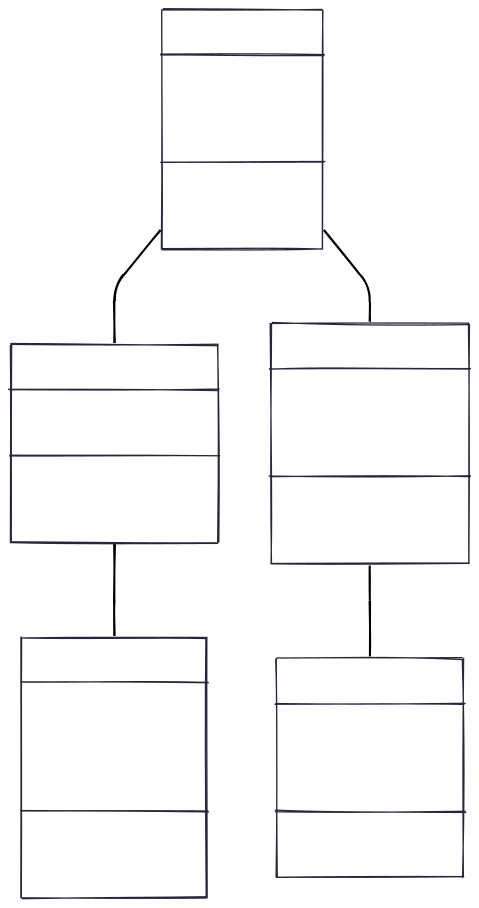
\includegraphics[width=0.7\textwidth]{diagrams/class-diagram.png}
    \caption{Class Diagram of the E-commerce System for SMEs}
\end{figure}

\textbf{Description of Main Classes:}

\begin{itemize}[]
    \item \textbf{User:} Represents all system users including shop owners and customers. Attributes include \textit{userID, name, email}, and methods like \textit{login(), logout(), updateProfile()}.
    \item \textbf{Product:} Represents items available for sale. Attributes include \textit{productID, name, price, stock}, and methods such as \textit{addProduct(), updateProduct(), removeProduct()}.
    \item \textbf{Order:} Captures customer orders. Attributes include \textit{orderID, date, status}, and methods like \textit{createOrder(), cancelOrder(), updateStatus()}.
    \item \textbf{Payment:} Handles transactions. Attributes include \textit{paymentID, amount, method}, with methods \textit{processPayment(), refundPayment()}.
    \item \textbf{Cart:} Represents the shopping cart. Attributes include \textit{cartID, items}, and methods like \textit{addItem(), removeItem(), calculateTotal()}.
\end{itemize}

\textbf{Object Diagram:} To illustrate the runtime scenario, consider an example where a customer places an order. The object diagram demonstrates the relationships between specific instances of classes at that point in time.

\begin{figure}[H]
    \centering
    \includegraphics[width=0.7\textwidth]{diagrams/sequence-diagram.png}
    \caption{Sequence Diagram Showing Customer Placing an Order}
\end{figure}

\textbf{Description of Objects:}

\begin{itemize}
    \item \textbf{customer1:User} – Represents a specific customer instance.
    \item \textbf{cart1:Cart} – The cart object linked to \textit{customer1}.
    \item \textbf{productA:Product, productB:Product} – Products added to \textit{cart1}.
    \item \textbf{order1:Order} – Generated when the customer confirms the purchase.
    \item \textbf{payment1:Payment} – Associated with \textit{order1} for transaction processing.
\end{itemize}

This modeling helps visualize the structure and behavior of the system, ensuring clear understanding of entity relationships and interactions before implementation. It also provides a foundation for refining class methods, attributes, and their interconnections during system design.

